\chapter{Identification of stakeholders and design concerns} \label{chp:identification-of-stakeholders-and-design-concerns}
	\begin{comment}
		An SDD shall identify the design stakeholders for the design subject.
		An SDD shall identify the design concerns of each identified design stakeholder.
		An SDD shall address each identified design concern.
		NOTE—An SDD can be used to satisfy the content guidelines for several types of design description as defined in
		ISO/IEC 15289:2006 [B25], by identifying their content guidelines as design concerns. The types of design
		descriptions are as follows: database design description (10.14),6 database detailed design description (10.15), highlevel
		software design description (10.22), interface description (10.27), low-level software design description (10.29),
		system description (10.71), and system element description (10.72).
	\end{comment}


\chapter{Templates} \label{Template viewpoint-view design label}
%\chapter{Template Design Viewpoint--View} \label{chp:template-vpv}
	\section{Viewpoint} \label{s:template-vpv-viewpoint}		
		\subsection{Context viewpoint} \label{s:template-vpv:context-viewpoint}
			\begin{comment}
				The Context viewpoint depicts services provided by a design subject with reference to an explicit context.
				That context is defined by reference to actors that include users and other stakeholders, which interact with
				the design subject in its environment. The Context viewpoint provides a “black box” perspective on the
				design subject.
				Services depict an inherently functional aspect or anticipated cases of use of the design subject (hence “use
				cases” in UML). Stratification of services and their descriptions in the form of scenarios of actors’
				interactions with the system provide a mechanism for adding detail. Services may also be associated with
				actors through information flows. The content and manner of information exchange with the environment
				implies additional design information and the need for additional viewpoints (see 5.10).
				A Deployment overlay to a Context view can be transformed into a Deployment view whenever the
				execution hardware platform is part of the design subject; for stand-alone software design, a Deployment
				overlay maps software entities onto externally available entities not subject of the current design effort.
				Similarly, work allocation to teams and other management perspectives are overlays in the design.
			\end{comment}
			
			\subsubsection{Design concerns} \label{s:template-vpv:design-concerns}
				\begin{comment}
					The purpose of the Context viewpoint is to identify a design subject’s offered services, its actors (users and
					other interacting stakeholders), to establish the system boundary and to effectively delineate the design
					subject’s scope of use and operation.
					Drawing a boundary separating a design subject from its environment, determining a set of services to be
					provided, and the information flows between design subject and its environment, is typically a key design
					decision. That makes this viewpoint applicable to most design efforts.
					When the system is portrayed as a black box, with internal decisions hidden, the Context view is often a
					starting point of design, showing what is to be designed functionally as the only available information
					about the design subject: a name and an associated set of externally identifiable services. Requirements
					analysis identifies these services with the specification of quality of service attributes, henceforth invoking
					many non-functional requirements. Frequently incomplete, a Context view is begun in requirements
					analysis. Work to complete this view continues during design.
				\end{comment}
				
			\subsubsection{Design elements} \label{s:template-vpv:design-elements}
				\begin{comment}
					Design entities: actors—external active elements interacting with the design subject, including users, other
					stakeholders and external systems, or other items; services—also called use cases; and directed information
					flows between the design subject, treated as a black box, and its actors associating actors with services.
					Flows capture the expected information content exchanged.
					Design relationships: receive output and provide input (between actors and the design subject).
					Design constraints: qualities of service; form and medium of interaction (provided to and received from)
					with environment.
				\end{comment}
				
			\subsubsection{Example languages} \label{s:template-vpv:example-languages}
				\begin{comment}
					Any black-box type diagrams can be used to realize the Context viewpoint. Appropriate languages include
					Structured Analysis [e.g., IDEF0 (IEEE Std 1320.1-1998 [B18]), Structured Analysis and Design 
					Technique (SADT) (Ross [B32]) or those of the DeMarco or Gane-Sarson variety], the Cleanroom’s black
					box diagrams, and UML use cases (OMG [B28]).
				\end{comment}
			
			
	\section{Composition viewpoint} \label{s:tempalte-vpv:composition-viewpoint}
		\begin{comment}
			The Composition viewpoint describes the way the design subject is (recursively) structured into constituent
			parts and establishes the roles of those parts.
		\end{comment}
		
		\subsection{Design concerns} \label{s:tempalte-vpv:design-concerns}
			\begin{comment}
				Software developers and maintainers use this viewpoint to identify the major design constituents of the
				design subject, to localize and allocate functionality, responsibilities, or other design roles to these
				constituents. In maintenance, it can be used to conduct impact analysis and localize the efforts of making
				changes. Reuse, on the level of existing subsystems and large-grained components, can be addressed as
				well. The information in a Composition view can be used by acquisition management and in project
				management for specification and assignment of work packages, and for planning, monitoring, and control
				of a software project. This information, together with other project information, can be used in estimating
				cost, staffing, and schedule for the development effort. Configuration management may use the information
				to establish the organization, tracking, and change management of emerging work products (see
				IEEE Std 12207-2008 [B21]).
			\end{comment}
			
		\subsection{Design elements} \label{s:template-vpv:design-elements}
			\begin{comment}
				Design entities: types of constituents of a system: subsystems, components, modules; ports and (provided
				and required) interfaces; also libraries, frameworks, software repositories, catalogs, and templates.
				Design relationships: composition, use, and generalization. The Composition viewpoint supports the
				recording of the part-whole relationships between design entities using realization, dependency,
				aggregation, composition, and generalization relationships. Additional design relationships are required and
				provided (interfaces), and the attachment of ports to components.
				Design attributes: For each design entity, the viewpoint provides a reference to a detailed description via
				the identification attribute. The attribute descriptions for identification, type, purpose, function, and
				definition attribute should be utilized.
			\end{comment}
		
			\subsubsection{Function attribute} \label{s:template-vpv:function-attribute}
				\begin{comment}
					A statement of what the entity does. The function attribute states the transformation applied by the entity to
					its inputs to produce the output. In the case of a data entity, this attribute states the type of information
					stored or transmitted by the entity.
					NOTE—This design attribute is retained for compatibility with IEEE Std 1016-1998.
				\end{comment}
			
			\subsubsection{Subordinates attribute} \label{s:template-vpv:subordinates-attribute}
				\begin{comment}
					The identification of all entities composing this entity. The subordinates attribute identifies the “composed
					of” relationship for an entity. This information is used to trace requirements to design entities and to
					identify parent/child structural relationships through a design subject.
					NOTE—This design attribute is retained for compatibility with IEEE Std 1016-1998. An equivalent capability is
					available through the composition relationship.
				\end{comment}
			
		\subsection{Example languages} \label{s:template-vpv:example-languages}
			\begin{comment}
				UML component diagrams (see OMG [B28]) cover this viewpoint. The simplest graphical technique used
				to describe functional system decomposition is a hierarchical decomposition diagram; such diagram can be
				used together with natural language descriptions of purpose and function for each entity, such as is
				provided by IDEF0 (IEEE Std 1320.1-1998 [B18]), the Structure Chart (Yourdon and Constantine [B38],
				and the HIPO Diagram. Run-time composition can also use structured diagrams (Page-Jones [B29]).
			\end{comment}
		
	\section{Logical viewpoint} \label{s:template-vpv:logiacl-viewpoint}
		\begin{comment}
			The purpose of the Logical viewpoint is to elaborate existing and designed types and their implementations
			as classes and interfaces with their structural static relationships. This viewpoint also uses examples of
			instances of types in outlining design ideas.
		\end{comment}
		
		\subsection{Design concerns} \label{s:template-vpv:design-concerns}
			\begin{comment}
				The Logical viewpoint is used to address the development and reuse of adequate abstractions and their
				implementations. For any implementation platform, a set of types is readily available for the domain
				abstractions of interest in a design subject, and a number of new types is to be designed, some of which
				may be considered for reuse. The main concern is the proper choice of abstractions and their expression in
				terms of existing types (some of which may had been specific to the design subject).
			\end{comment}
			
		\subsection{Design elements} \label{s:template-vpv:design-elements}
			\begin{comment}
				Design entities: class, interface, power type, data type, object, attribute, method, association class, template,
				and namespace.
				Design relationships: association, generalization, dependency, realization, implementation, instance of,
				composition, and aggregation.
				Design attributes: name, role name, visibility, cardinality, type, stereotype, redefinition, tagged value,
				parameter, and navigation efficiency.
				Design constraints: value constraints, relationships exclusivity constraints, navigability, generalization sets,
				multiplicity, derivation, changeability, initial value, qualifier, ordering, static, pre-condition, post-condition,
				and generalization set constraints.
			\end{comment}
		
		\subsection{Example languages} \label{s:template-vpv:example-languages}
			\begin{comment}
				UML class diagrams and UML object diagrams (showing objects as instances of their respective classes)
				(OMG [B28]). Lattices of types and references to implemented types are commonly used as supplementary
				information.
			\end{comment}
			
	\section{Dependency viewpoint} \label{s:template-vpv:dependency-viewpoint}
		\begin{comment}
			The Dependency viewpoint specifies the relationships of interconnection and access among entities. These
			relationships include shared information, order of execution, or parameterization of interfaces.
		\end{comment}
		
		\subsection{Design concerns} \label{s:template-vpv:design-concerns}
			\begin{comment}
				A Dependency view provides an overall picture of the design subject in order to assess the impact of
				requirements or design changes. It can help maintainers to isolate entities causing system failures or
				resource bottlenecks. It can aid in producing the system integration plan by identifying the entities that are
				needed by other entities and that must be developed first. This description can also be used by integration
				testing to aid in the production of integration test cases.
			\end{comment}

\chapter{Context Viewpoint Template} \label{chp:context-viewpoint-template}
	\begin{comment}
		The Context viewpoint depicts services provided by a design subject with reference to an explicit context.
		That context is defined by reference to actors that include users and other stakeholders, which interact with
		the design subject in its environment. The Context viewpoint provides a “black box” perspective on the
		design subject.
		Services depict an inherently functional aspect or anticipated cases of use of the design subject (hence “use
		cases” in UML). Stratification of services and their descriptions in the form of scenarios of actors’
		interactions with the system provide a mechanism for adding detail. Services may also be associated with
		actors through information flows. The content and manner of information exchange with the environment
		implies additional design information and the need for additional viewpoints (see 5.10).
		A Deployment overlay to a Context view can be transformed into a Deployment view whenever the
		execution hardware platform is part of the design subject; for stand-alone software design, a Deployment
		overlay maps software entities onto externally available entities not subject of the current design effort.
		Similarly, work allocation to teams and other management perspectives are overlays in the design.
	\end{comment}
	This viewpoint identifies basic features of \emph{Computational Library}, main user and example of input data.
	\section{Design concerns} \label{s:context-viewpoint-template:design-concerns}
		\begin{comment}
			The purpose of the Context viewpoint is to identify a design subject’s offered services, its actors (users and
			other interacting stakeholders), to establish the system boundary and to effectively delineate the design
			subject’s scope of use and operation.
			Drawing a boundary separating a design subject from its environment, determining a set of services to be
			provided, and the information flows between design subject and its environment, is typically a key design
			decision. That makes this viewpoint applicable to most design efforts.
			When the system is portrayed as a black box, with internal decisions hidden, the Context view is often a
			starting point of design, showing what is to be designed functionally as the only available information
			about the design subject: a name and an associated set of externally identifiable services. Requirements
			analysis identifies these services with the specification of quality of service attributes, henceforth invoking
			many non-functional requirements. Frequently incomplete, a Context view is begun in requirements
			analysis. Work to complete this view continues during design.
		\end{comment}
		
		\begin{concerns}{Library use--cases}{API}
			\begin{figure}[!htp]
				\centering
				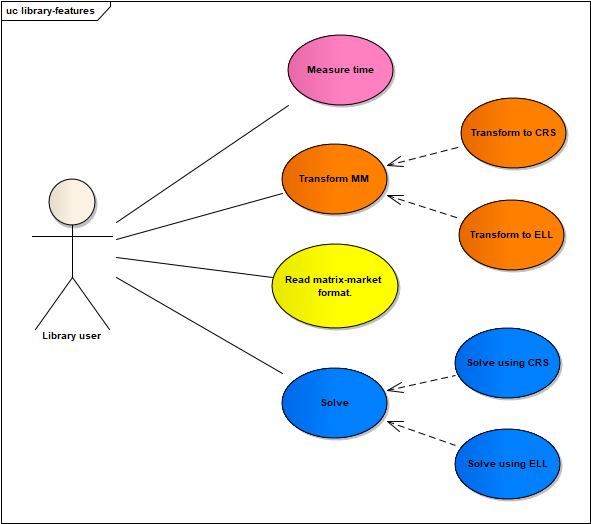
\includegraphics[scale=0.6]{others/img/library-features}
				\caption{Use--case diagram of computation library features.}
			\end{figure}
		\end{concerns}
		\clearpage
		\begin{concerns}{Example \gls{MM} file}{Input}
			\lstinputlisting[basicstyle=\tiny]{others/cage4.mtx}
		\end{concerns}
		\clearpage
		\begin{concerns}{Basic usage of library features}{API}
			\begin{figure}[!htp]
				\centering
				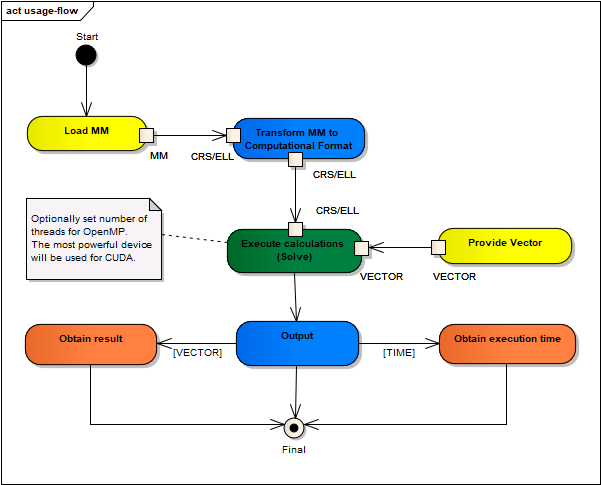
\includegraphics[scale=0.6]{others/img/usage-flow}
				\caption{General usage--flow of application.}
			\end{figure}
		\end{concerns}
	\section{Design elements} \label{s:context-viewpoint-template:design-elements}
		\begin{comment}
			Design entities: actors—external active elements interacting with the design subject, including users, other
			stakeholders and external systems, or other items; services—also called use cases; and directed information
			flows between the design subject, treated as a black box, and its actors associating actors with services.
			Flows capture the expected information content exchanged.
			
			Design relationships: receive output and provide input (between actors and the design subject).
			
			Design constraints: qualities of service; form and medium of interaction (provided to and received from)
			with environment.
		\end{comment}
	
		\begin{design-element}{User}{Actor}
			User of the library can be a programmer, researcher or scientist.
		\end{design-element}
	
		\begin{design-element}{\gls{MM} file}{Constraints}
			Following storage-data types are supported:
			\begin{itemize}
				\item general
				\item symmetric
			\end{itemize}
			Following value data types are supported:
			\begin{itemize}
				\item real
				\item pattern
				\item integer
			\end{itemize}
		\end{design-element}
	%\section{Example languages} \label{s:context-viewpoint-template:example-languages}
		\begin{comment}
			Any black-box type diagrams can be used to realize the Context viewpoint. Appropriate languages include
			Structured Analysis [e.g., IDEF0 (IEEE Std 1320.1-1998 [B18]), Structured Analysis and Design 
			Technique (SADT) (Ross [B32]) or those of the DeMarco or Gane-Sarson variety], the Cleanroom’s black
			box diagrams, and UML use cases (OMG [B28]).
		\end{comment}
\chapter{Composition Viewpoint} \label{chp:composition-viewpoint-template}
	\begin{comment}
		The Composition viewpoint describes the way the design subject is (recursively) structured into constituent
		parts and establishes the roles of those parts.
	\end{comment}
	This viewpoint identifies major design concepts. It explains composition of provided solution, distinguishing location for each class and routines.
	\section{Design concerns} \label{s:composition-viewpoint-template:design-concerns}
		\begin{comment}
			Software developers and maintainers use this viewpoint to identify the major design constituents of the
			design subject, to localize and allocate functionality, responsibilities, or other design roles to these
			constituents. In maintenance, it can be used to conduct impact analysis and localize the efforts of making
			changes. Reuse, on the level of existing subsystems and large-grained components, can be addressed as
			well. The information in a Composition view can be used by acquisition management and in project
			management for specification and assignment of work packages, and for planning, monitoring, and control
			of a software project. This information, together with other project information, can be used in estimating
			cost, staffing, and schedule for the development effort. Configuration management may use the information
			to establish the organization, tracking, and change management of emerging work products (see
			IEEE Std 12207-2008 [B21]).
		\end{comment}
		
		\begin{concerns}{Library structure}{Maintenance}
			In order to manage different dependencies library is divided into parts depending on their role and way of implementation. Each new project containing computational routines should contain new implementation of \gls{CRS} and \gls{ELL} abstract solvers and specific for the platform measurement tool. New platform requires also corresponding test project.
		\end{concerns}
	\section{Design elements} \label{s:composition-viewpoint-template:design-elements}
		\begin{comment}
			Design entities: types of constituents of a system: subsystems, components, modules; ports and (provided
			and required) interfaces; also libraries, frameworks, software repositories, catalogs, and templates.
			
			Design relationships: composition, use, and generalization. The Composition viewpoint supports the
			recording of the part-whole relationships between design entities using realization, dependency,
			aggregation, composition, and generalization relationships. Additional design relationships are required and
			provided (interfaces), and the attachment of ports to components.
			
			Design attributes: For each design entity, the viewpoint provides a reference to a detailed description via
			the identification attribute. The attribute descriptions for identification, type, purpose, function, and
			definition attribute should be utilized.
		\end{comment}	
		\begin{design-element}{Responsibilities and structure design}{Structure}
				\begin{table}[!hp]
				\centering
				\caption{Components of \emph{Computational Library}}
				\label{tab:components-comp}
				\resizebox{\textwidth}{!}{
					\begin{tabular}{|l|l|l|l|}
						\hline
						\textbf{Project} & \textbf{Description} & \textbf{Dependencies} & \textbf{References} \\ \hline
						\texttt{sspp.common} & \begin{tabular}[c]{@{}l@{}}Contains basic routines for reading MM, \\ transforming between \gls{CRS} and \gls{ELL}.\\ Additionaly contains routines for calculating \\ matrix-vector dot product in serial.\end{tabular} & None & None \\ \hline
						\texttt{sspp.common.tests} & \begin{tabular}[c]{@{}l@{}}Contains all unit-test cases for \texttt{sspp.common}\\ project.\end{tabular} & \texttt{sspp.common} & \begin{tabular}[c]{@{}l@{}}\texttt{gtest}\\ \texttt{gmock}\end{tabular} \\ \hline
						\texttt{sspp.cuda} & \begin{tabular}[c]{@{}l@{}}Implementation of computation routines\\  using \gls{cuda}.\end{tabular} & \texttt{sspp.common} & \gls{cuda} Toolkit \\ \hline
						\texttt{sspp.cuda.tests} & \begin{tabular}[c]{@{}l@{}}Contains all unit-test cases for \texttt{sspp.cuda} \\ project.\end{tabular} & \begin{tabular}[c]{@{}l@{}}\texttt{sspp.common}\\ \texttt{sspp.cuda}\end{tabular} & \begin{tabular}[c]{@{}l@{}}\texttt{gtest}\\ \texttt{gmock}\\ \gls{cuda} Toolkit\end{tabular} \\ \hline
						\texttt{sspp.openmp} & \begin{tabular}[c]{@{}l@{}}Implementation of computation routines\\  using \gls{openmp}.\end{tabular} & \texttt{sspp.common} & \gls{openmp} \\ \hline
						\texttt{sspp.openmp.tests} & \begin{tabular}[c]{@{}l@{}}Contains all unit-test cases for \texttt{sspp.openmp}\\ project.\end{tabular} & \begin{tabular}[c]{@{}l@{}}\texttt{sspp.common}\\ \texttt{sspp.openmp}\end{tabular} & \begin{tabular}[c]{@{}l@{}}\gls{openmp}\\ \texttt{gtest}\\ \texttt{gmock}\end{tabular} \\ \hline
						\texttt{sspp.performance.tests} & Contains all performance test for all routines. & All & \begin{tabular}[c]{@{}l@{}}\gls{openmp}\\ \texttt{gtest}\\ \texttt{gmock}\\ \gls{cuda} Toolkit\end{tabular} \\ \hline
					\end{tabular}
				}
			\end{table}
		\end{design-element}
	%	\subsection{Function attribute} \label{s:composition-viewpoint-template:function-attribute}
			\begin{comment}
				A statement of what the entity does. The function attribute states the transformation applied by the entity to
				its inputs to produce the output. In the case of a data entity, this attribute states the type of information
				stored or transmitted by the entity.
				
				NOTE—This design attribute is retained for compatibility with IEEE Std 1016-1998.
			\end{comment}
		
		%\subsection{Subordinates attribute} \label{s:subordinates-viewpoint-template:function-attribute}
			\begin{comment}
				The identification of all entities composing this entity. The subordinates attribute identifies the “composed
				of” relationship for an entity. This information is used to trace requirements to design entities and to
				identify parent/child structural relationships through a design subject.
			
				NOTE—This design attribute is retained for compatibility with IEEE Std 1016-1998. An equivalent capability is
				available through the composition relationship.
			\end{comment}
			
%	\section{Example languages} \label{s:composition-viewpoint-template:example-languages}
		\begin{comment}
			UML component diagrams (see OMG [B28]) cover this viewpoint. The simplest graphical technique used
			to describe functional system decomposition is a hierarchical decomposition diagram; such diagram can be
			used together with natural language descriptions of purpose and function for each entity, such as is
			provided by IDEF0 (IEEE Std 1320.1-1998 [B18]), the Structure Chart (Yourdon and Constantine [B38],
			and the HIPO Diagram. Run-time composition can also use structured diagrams (Page-Jones [B29]).
		\end{comment}
\chapter{Logical Viewpoint} \label{chp:logical-viewpoint-template}
	\begin{comment}
		The purpose of the Logical viewpoint is to elaborate existing and designed types and their implementations
		as classes and interfaces with their structural static relationships. This viewpoint also uses examples of
		instances of types in outlining design ideas.
	\end{comment}
	
	\section{Design concerns} \label{s:logical-viewpoint-template:design-concerns}
		\begin{comment}
			The Logical viewpoint is used to address the development and reuse of adequate abstractions and their
			implementations. For any implementation platform, a set of types is readily available for the domain
			abstractions of interest in a design subject, and a number of new types is to be designed, some of which
			may be considered for reuse. The main concern is the proper choice of abstractions and their expression in
			terms of existing types (some of which may had been specific to the design subject).
		\end{comment}
		The logical viewpoint is used to address the development and reuse of adequate abstractions and their implementations.
	\section{Design elements} \label{s:logical-viewpoint-template:design-elements}
		\begin{comment}
			Design entities: class, interface, power type, data type, object, attribute, method, association class, template,
			and namespace.
			
			Design relationships: association, generalization, dependency, realization, implementation, instance of,
			composition, and aggregation.
			
			Design attributes: name, role name, visibility, cardinality, type, stereotype, redefinition, tagged value,
			parameter, and navigation efficiency.
			
			Design constraints: value constraints, relationships exclusivity constraints, navigability, generalization sets,
			multiplicity, derivation, changeability, initial value, qualifier, ordering, static, pre-condition, post-condition,
			and generalization set constraints.
		\end{comment}
		
		\begin{design-element}{Sparse matrix formats}{Class Hierarchy}
			Diagram \ref{fig:sparse-matrices} presents all sparse matrix formats supported by \emph{Computational Library}. Distinguishing: \gls{CRS}, \gls{ELL} and \gls{MM}. All of those matrices are implemented as \emph{C++} templates, which allows user to specify the type of matrix values. This approach allows to extend existing classes to complex types.
			\begin{figure}[!hp]
				\centering
				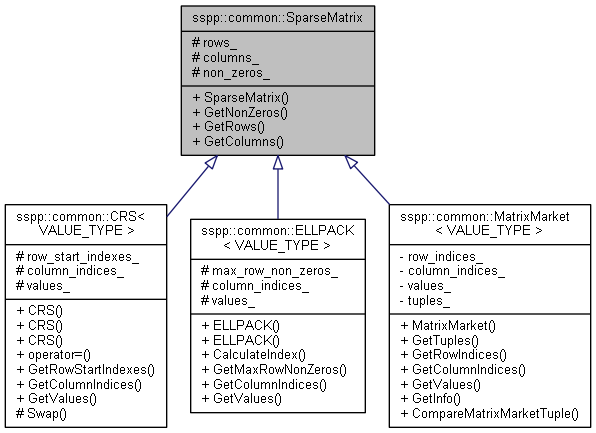
\includegraphics[scale=0.6]{others/img/sparse}
				\caption{Sparse matrix hierarchy classes.}
				\label{fig:sparse-matrices}
			\end{figure}
		\end{design-element}
	
		\begin{design-element}{\glsdesc{MM} Reader}{Collaboration}
			Diagram \ref{fig:mm-reader} presents function calls according to supported storage types and data types. As it is visualized reading \gls{MM} format is a two steps process. 
			\begin{figure}[!hp]
				\centering
				
\includegraphics[width=\textwidth]{others/img/matrix-market-reader}
				\caption{\glsdesc{MM} format collaboration diagram.}
				\label{fig:mm-reader}
			\end{figure}
		\end{design-element}
	
		\begin{design-element}{\glsdesc{CRS} Transformer}{Collaboration}
			Diagram \ref{fig:crs-transformer} describes all the included classes and routines during transformation from \gls{MM} to \gls{CRS} formats.
			\begin{figure}[!hp]
				\centering
				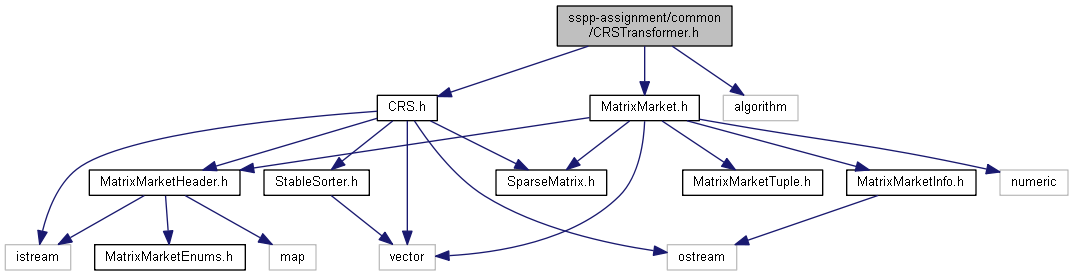
\includegraphics[width=\textwidth]{others/img/crs-transformer}
				\caption{\gls{CRS} Transformer collaboration diagram.}
				\label{fig:crs-transformer}
			\end{figure}
		\end{design-element}
		\clearpage
		\begin{design-element}{\glsdesc{ELL} Transformer}{Collaboration}
			Diagram \ref{fig:ell-transformer} describes all the included classes and routines during transformation from \gls{MM} to \gls{ELL} formats.
			\begin{figure}[!hp]
				\centering
				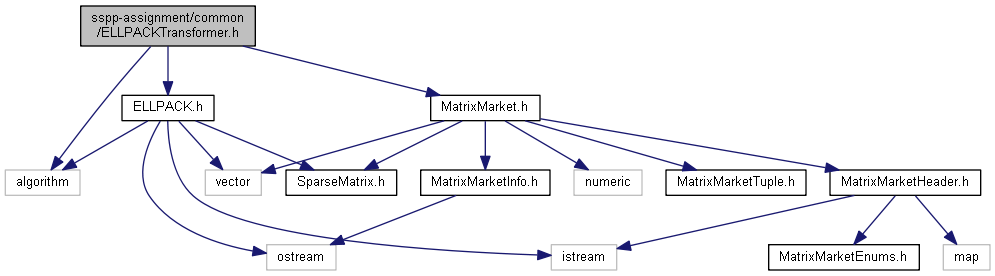
\includegraphics[width=\textwidth]{others/img/ellpack-transformer}
				\caption{\gls{ELL} Transformer collaboration diagram.}
				\label{fig:ell-transformer}
			\end{figure}
		\end{design-element}
	
		\begin{design-element}{Abstract \glsdesc{CRS} Solver}{Class hierarchy}
			Diagram \ref{fig:crs-solver} presents Abstract \gls{CRS} Solver class which is written using \emph{C++} templates for providing high extendability of library. We can distinguish tree different implementations for serial, \gls{cuda} and \gls{openmp} frameworks. Last one contains additional function to tune number of threads. 
			\begin{figure}[!hp]
				\centering
				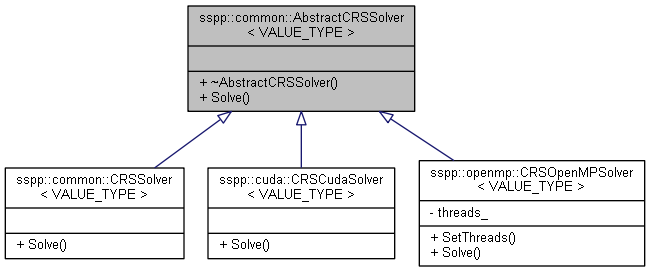
\includegraphics[scale=0.6]{others/img/abstract-crs-solver}
				\caption{Abstract \glsdesc{CRS} Solver class diagram.}
				\label{fig:crs-solver}
			\end{figure}
		\end{design-element}
		\clearpage
		\begin{design-element}{Abstract \glsdesc{ELL} Solver}{Class hierarchy}
				Diagram \ref{fig:ell-solver} presents Abstract \gls{ELL} Solver class which is written using \emph{C++} templates for providing high extendability of library. We can distinguish tree different implementations for serial, \gls{cuda} and \gls{openmp} frameworks. Last one contains additional function to tune number of threads. 
			\begin{figure}[!hp]
				\centering
				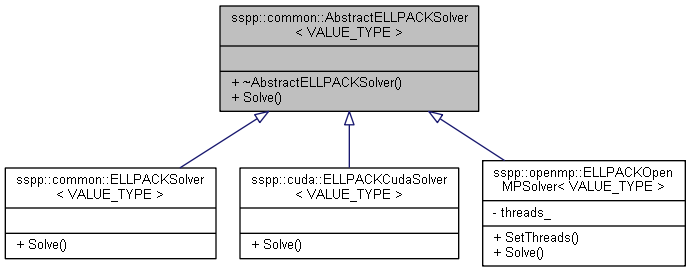
\includegraphics[scale=0.6]{others/img/abstract-elpack-solver}
				\caption{Abstract \glsdesc{ELL} Solver class diagram.}
				\label{fig:ell-solver}
			\end{figure}
		\end{design-element}
	
		\begin{design-element}{Abstract Stopwatch}{Collaboration}
			Abstract stopwatch presented in Diagram \ref{fig:abstract-stopwatch} is implemented in tree different ways depending on used framework. As we can see \texttt{ChronoStopwatch} is used for serial code, \texttt{OpenMPStopwatch} is used in \gls{openmp} module and the last \texttt{CUDAStopwatch} is used in \gls{cuda} module.
			\begin{figure}[!hp]
				\centering
				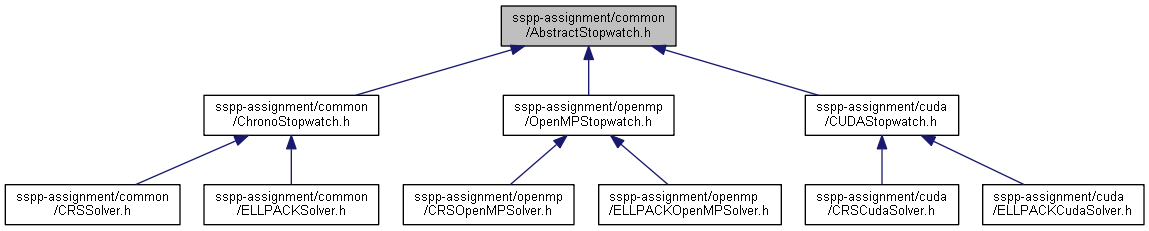
\includegraphics[width=\textwidth]{others/img/abstract-stopwatch-calls}
				\caption{Abstract stopwatch routines.}
				\label{fig:abstract-stopwatch}
			\end{figure}
		\end{design-element}
%	\section{Example languages} \label{s:logical-viewpoint-template:example-languages}
		\begin{comment}
			UML class diagrams and UML object diagrams (showing objects as instances of their respective classes)
			(OMG [B28]). Lattices of types and references to implemented types are commonly used as supplementary
			information.
		\end{comment}
\chapter{Dependency Viewpoint Template} \label{chp:dependency-viewpoint-template}
	\begin{comment}
		The Dependency viewpoint specifies the relationships of interconnection and access among entities. These
		relationships include shared information, order of execution, or parameterization of interfaces.
	\end{comment}
	
	\section{Design concerns} \label{s:dependency-viewpoint-template:design-concerns}
		\begin{comment}
			A Dependency view provides an overall picture of the design subject in order to assess the impact of
			requirements or design changes. It can help maintainers to isolate entities causing system failures or
			resource bottlenecks. It can aid in producing the system integration plan by identifying the entities that are
			needed by other entities and that must be developed first. This description can also be used by integration
			testing to aid in the production of integration test cases.
		\end{comment}
	
	\section{Design elements} \label{s:dependency-viewpoint-template:design-elements}
		\begin{comment}
			Design entities: subsystem, component, and module.
			
			Design relationships: uses, provides, and requires.
			
			Design attribute: name (4.6.2.1), type (4.6.2.2), purpose (4.6.2.3), dependencies (5.5.2.1), and resources.
			These attributes should be provided for all design entities.
		\end{comment}
	
		\subsection{Dependencies attribute} \label{s:dependency-viewpoint-template:dependencies-attribute}
			\begin{comment}
				A description of the relationships of this entity with other entities. The dependencies attribute identifies the
				uses or requires the presence of relationship for an entity. This attribute is used to describe the nature of
				each interaction including such characteristics as timing and conditions for interaction. The interactions
				involve the initiation, order of execution, data sharing, creation, duplicating, usage, storage, or destruction
				of entities.
				NOTE—This design entity attribute is retained for compatibility with IEEE Std 1016-1998.
			\end{comment}
			
	\section{Example languages} \label{s:dependency-viewpoint-template:example-languages}
		\begin{comment}
			UML component diagrams and UML package diagrams showing dependencies among subsystems (OMG
			[B28]).
		\end{comment}
\chapter{Information Viewpoint Template} \label{chp:information-viewpoint-template}
	\begin{comment}
		The Information viewpoint is applicable when there is a substantial persistent data content expected with
		the design subject.
	\end{comment}
	
	\section{Design concerns} \label{s:information-viewpoint-template:design-concerns}
		\begin{comment}
			Key concerns include persistent data structure, data content, data management strategies, data access
			schemes, and definition of metadata.
		\end{comment}
	
	\section{Design elements} \label{s:information-viewpoint-template:design-elements}
		\begin{comment}
			Design entities: data items, data types and classes, data stores, and access mechanisms.
			
			Design relationships: association, uses, implements. Data attributes, their constraints and static
			relationships among data entities, aggregates of attributes, and relationships.
			
			Design attributes: persistence and quality properties.
		\end{comment}
	
		\subsection{Data attribute} \label{s:information-viewpoint-template:data-attribute}
			\begin{comment}
				A description of data elements internal to the entity. The data attribute describes the method of
				representation, initial values, use, semantics, format, and acceptable values of internal data. The description
				of data may be in the form of a data dictionary that describes the content, structure, and use of all data
				elements. Data information should describe everything pertaining to the use of data or internal data
				structures by this entity. It should include data specifications such as formats, number of elements, and
				initial values. It should also include the structures to be used for representing data such as file structures,
				arrays, stacks, queues, and memory partitions.
				
				The meaning and use of data elements should be specified. This description includes such things as static
				versus dynamic, whether it is to be shared by transactions, used as a control parameter, or used as a value,
				loop iteration count, pointer, or link field. In addition, data information should include a description of data
				validation needed for the process.
				
				NOTE—This design attribute is retained for compatibility with IEEE Std 1016-1998.
			\end{comment}
			
	\section{Example languages} \label{s:information-viewpoint-template:example-languages}
		\begin{comment}
			IDEF1X (IEEE Std 1320.2™-1998 [B19]), UML class diagrams (OMG [B28]).
		\end{comment}
\chapter{Pattern use Viewpoint Template} \label{chp:pattern-use-viewpoint-template}
	\begin{comment}
		This viewpoint addresses design ideas (emergent concepts) as collaboration patterns involving abstracted
		roles and connectors.
	\end{comment}
	
	\section{Design concerns} \label{s:pattern-use-viewpoint-template:design-concerns}
		\begin{comment}
			Key concerns include reuse at the level of design ideas (design patterns), architectural styles, and
			framework templates.
		\end{comment}
	
	\section{Design elements} \label{s:pattern-use-viewpoint-template:design-elements}
		\begin{comment}
			Design entities: collaboration, class, connector, role, framework template, and pattern.
			
			Design relationships: association, collaboration use, and connector.
			
			Design attributes: name.
			
			Design constraints: collaboration constraints.
		\end{comment}
	
	\section{Example languages} \label{s:pattern-use-viewpoint-template:example-languages}
		\begin{comment}
			UML composite structure diagram and a combination of the UML class diagram and the UML package
			diagram (OMG [B28]).
		\end{comment}
\chapter{Interface Viewpoint Template} \label{chp:interface-viewpoint-template}
	\begin{comment}
		The Interface viewpoint provides information designers, programmers, and testers the means to know how
		to correctly use the services provided by a design subject. This description includes the details of external
		and internal interfaces not provided in the SRS. This viewpoint consists of a set of interface specifications
		for each entity.
		NOTE—User interfaces are addressed separately.
	\end{comment}
	
	\section{Design concerns} \label{s:interface-viewpoint-template:design-concerns}
		\begin{comment}
			An Interface view description serves as a binding contract among designers, programmers, customers, and
			testers. It provides them with an agreement needed before proceeding with the detailed design of entities.
			The interface description is used by technical writers to produce customer documentation or may be used
			directly by customers. In the latter case, the interface description could result in the production of a human
			interface view.
			
			Designers, programmers, and testers often use design entities that they did not develop. These entities can
			be reused from earlier projects, contracted from an external source, or produced by other developers. The
			interface description establishes an agreement among designers, programmers, and testers about how
			cooperating entities will interact. Each entity interface description should contain everything another
			designer or programmer needs to know to develop software that interacts with that entity. A clear
			description of entity interfaces is essential on a multi-person development for smooth integration and ease
			of maintenance.
		\end{comment}
	
	\section{Design elements} \label{s:interface-viewpoint-template:design-elements}
		\begin{comment}
			The attributes for identification (4.6.2.1), function (5.3.2.1), and interface (5.8.2.1) should be provided for
			all design entities.
		\end{comment}
	
		\subsection{Interface attribute} \label{s:interface-viewpoint-template:interface-attribute}
			\begin{comment}
				A description of how other entities interact with this entity. The interface attribute describes the methods of
				interaction and the rules governing those interactions. Methods of interaction include the mechanisms for
				invoking or interrupting the entity, for communicating through parameters, common data areas or
				messages, and for direct access to internal data. The rules governing the interaction include the
				communications protocol, data format, acceptable values, and the meaning of each value.
				
				This attribute provides a description of the input ranges, the meaning of inputs and outputs, the type and
				format of each input or output, and output error codes. For information systems, it should include inputs,
				screen formats, and a complete description of the interactive language.
				
				NOTE—This design attribute is retained for compatibility with IEEE Std 1016-1998
			\end{comment}
			
	\section{Example languages} \label{s:interface-viewpoint-template:example-languages}
		\begin{comment}
			Interface definition languages (IDL), UML component diagram (OMG [B28]). In case of user interfaces
			the Interface view should include screen formats, valid inputs, and resulting outputs. For data-driven
			entities, a data dictionary should be used to describe the data characteristics. Those entities that are highly
			visible to a user and involve the details of how the customer should perceive the system should include a
			functional model, scenarios for use, detailed feature sets, and the interaction language.
		\end{comment}
\chapter{Structure Viewpoint Template} \label{chp:structure-viewpoint-template}
	\begin{comment}
		The Structure viewpoint is used to document the internal constituents and organization of the design subject
		in terms of like elements (recursively).
	\end{comment}
	
	\section{Design concerns} \label{s:structure-viewpoint-template:design-concerns}
		\begin{comment}
			Compositional structure of coarse-grained components and reuse of fine-grained components.
		\end{comment}
	
	\section{Design elements} \label{s:structure-viewpoint-template:design-elements}
		\begin{comment}
			Design entities: port, connector, interface, part, and class.
			
			Design relationships: connected, part of, enclosed, provided, and required.
			
			Design attributes: name, type, purpose, and definition.
			
			Design constraints: interface constraints, reusability constraints, and dependency constraints.
		\end{comment}
	
	\section{Example languages} \label{s:structure-viewpoint-template:example-languages}
		\begin{comment}
			UML composite structure diagram, UML class diagram, and UML package diagram (OMG [B28]).
		\end{comment}
\chapter{Interaction Viewpoint Template} \label{chp:interaction-viewpoint-template}
	\begin{comment}
		The Interaction viewpoint defines strategies for interaction among entities, regarding why, where, how, and
		at what level actions occur.
	\end{comment}
	
	\section{Design concerns} \label{s:interaction-viewpoint-template:design-concerns}
		\begin{comment}
			For designers. this includes evaluating allocation of responsibilities in collaborations, especially when
			adapting and applying design patterns; discovery or description of interactions in terms of messages among
			affected objects in fulfilling required actions; and state transition logic and concurrency for reactive,
			interactive, distributed, real-time, and similar systems.
		\end{comment}
	
	\section{Design elements} \label{s:interaction-viewpoint-template:design-elements}
		\begin{comment}
			Classes, methods. states, events, signals, hierarchy, concurrency, timing, and synchronization.
		\end{comment}
	
	\section{Example languages} \label{s:interaction-viewpoint-template:example-languages}
		\begin{comment}
			UML composite structure diagram, UML interaction diagram (OMG [B28]).
		\end{comment}
\chapter{State Dynamics Viewpoint Template} \label{chp:state-dynamics-viewpoint-template}
	\begin{comment}
		Reactive systems and systems whose internal behavior is of interest use this viewpoint.
	\end{comment}
	
	\section{Design concerns} \label{s:state-dynamics-viewpoint-template:design-concerns}
		\begin{comment}
			System dynamics including modes, states, transitions, and reactions to events.
		\end{comment}
	
	\section{Design elements} \label{s:state-dynamics-viewpoint-template:design-elements}
		\begin{comment}
			Design entities: event, condition, state, transition, activity, composite state, submachine state, critical
			region, and trigger.
			
			Design relationships: part-of, internal, effect, entry, exit, and attached to.
			
			Design attributes: name, completion, active, initial, and final.
			
			Design constraints: guard conditions, concurrency, synchronization, state invariant, transition constraint,
			and protocol.
		\end{comment}
	
	\section{Example languages} \label{s:state-dynamics-viewpoint-template:example-languages}
		\begin{comment}
			UML state machine diagram (OMG [B28]), Harel statechart, state transition table (matrix), automata, Petri
			net.
		\end{comment}
\chapter{Algorithm Viewpoint}
\label{ch:algorithm-viewpoint}
\begin{comment}
	The detailed design description of operations (such as methods and functions), the internal details and logic of each design entity.
\end{comment}
	
	\section{Design concerns}
	\label{sec:algorithm-viewpoint:design-concerns}
	The Algorithm viewpoint provides details of algorithms in regard to time-space performance and processing logic prior to implementation, and to aid in producing unit test plans.
	\begin{comment}
		The Algorithm viewpoint provides details needed by programmers, analysts of algorithms in regard to	time-space performance and processing logic prior to implementation, and to aid in producing unit test plans.
	\end{comment}
	
	\begin{concerns}{Transforming \gls{MM} to \gls{CRS}}{Structure}
		Below pseudocode assumes, that \texttt{tuples} is an array of \gls{MM} entry, containing row and column coordinates, as well as value of the entry. 
		\begin{lstlisting}[language=C++,caption={Pseudocode of transforming algorithm from \gls{MM} to \gls{CRS} format.}]
crs function transform_to_CRS()
	sort tuples by row and within each row by column;
	values[non_zeros];
	row_start_indexes[rows + 1];
	columnd_indices[non_zeros];
	set row_start_indexes_index to 0;
	set non_zeros_index to 1;
	set row_start_indexes[row_start_indexes_index++] to 0;
	
	while (row_start_indexes_index < rows + 1 and non_zeros_index < non_zeros) do
		begin
			set column_indices[non_zeros_index - 1] to tuples[non_zeros_index - 1]->column_indice;
			set values[non_zeros_index - 1] to tuples[non_zeros_index - 1]->value;
			set row_indices_diff to tuples[non_zeros_index].row_indice - tuples[non_zeros_index - 1].row_indice;
			if (row_indices_diff != 0) then
				set row_start_indexes[row_start_indexes_index++] to non_zeros_index;
				if (row_indices_diff > 1) then
					for (i = 0; i < row_indices_diff - 1; ++i) do
						set row_start_indexes[row_start_indexes_index++] to non_zeros_index;
					end for
				end if
			end if
			set non_zeros_index to non_zeros_index + 1;
		end
	for (i = row_start_indexes_index; i < rows; ++i) do 
		set row_start_indexes[row_start_indexes_index++] to non_zeros_index;
	end for
	set row_start_indexes[row_start_indexes_index++] to non_zeros_index;
	set column_indices[non_zeros_index - 1] to tuples[non_zeros_index - 1]->column_indice;
	set values[non_zeros_index - 1] to tuples[non_zeros_index - 1]->value;
	return crs(rows, columns, non_zeros, row_start_indexes, column_indices, values);
end function
		\end{lstlisting}
	\end{concerns}

	\begin{concerns}{Transforming \gls{MM} to \gls{ELL}}{}
		Below pseudocode assumes, that \texttt{tuples} is an array of \gls{MM} entry, containing row and column coordinates, as well as value of the entry.
		\begin{lstlisting}[language=C++, caption={Pseudocode of transforming algorithm from \gls{MM} to \gls{ELL} format.}]
ellpack function transform_to_ELLPACK()
	create aux with max_nonzeros per row in entries;
	find row in aux_vector with maximum non_zeros and save to max_non_zeros;
	values[max_non_zeros * rows];
	column_indices[max_non_zeros * rows];
	
	for (i = 0; i < non_zeros; i++) do
		set index to max_row_non_zeros * tuples[i]->row_indice + aux_vector[tuples[i]->row_indice] - 1;
		set column_indices[index] to tuples->column_indice;
		set values[index] to tuples->value;
		--aux_vector[tuples[i]->row_indice];
	end for
	
	return ellpack(rows, columns, non_zeros, max_non_zeros, column_indices, values);
end function
		\end{lstlisting}
	\end{concerns}

	\begin{concerns}{Calculations of \gls{CRS}--vector dot product in serial}{}
		\begin{lstlisting}[language=C++, caption={Pseudocode of \gls{CRS}--vector dot product in serial.}]
void function sequential_CRS()
	for (i = 0; i < rows; i++) {
		set tmp to 0;
		for (j = row_start_indexes[i]; j < row_start_indexes[i + 1]; j++) do
			set tmp to tmp + values[j] * vector[column_indices[j]];
		end for
		set result[i] to tmp;
	}
end function
		\end{lstlisting}
	\end{concerns}
	\clearpage
	\begin{concerns}{Calculations of \gls{ELL}--vector dot product in serial}{}
		\begin{lstlisting}[language=C++, caption={Pseudocode of \gls{ELL}--vector dot product in serial.}]
void function sequential_ELLPACK() 
	for (i = 0; i < rows; i++) do
		set tmp to 0;
		for (j = 0; j < max_non_zeros; j++) do
			set tmp to tmp + values[i][j] * vector[column_indices[i][j]];
		end for
		set result[i] to tmp;
	end for
end function
		\end{lstlisting}
	\end{concerns}	

	\begin{concerns}{Calculations of \gls{CRS}--vector dot product with \gls{openmp}}{}
		
		For effective usage of threads, each thread should be assigned with equal number of operations to perform. Following solution distributes equally chunks of rows between active threads. This solution is the most efficient, if each row in matrix contains same number of nonzeros. In worst case scenario, if nonzeros are not equally distributed in matrix, this algorithm can assign whole load to a single thread, causing other threads to wait. 
		\begin{lstlisting}[language=C++, caption={Pseudocode of \gls{CRS}--vector dot product with \gls{openmp}.}]
void function parallel()
	set threadId to current_thread_id;
	set threads to number_of_threads;
	set lowerBoundary to rows * threadId / threads;
	set upperBoundary to rows * (threadId + 1) / threads;
	#execute in parallel
	for (i = lowerBoundary; i < upperBoundary; i++) do
		set sum to 0;
		for (j = row_start_indexes[i]; j < row_start_indexes[i + 1]; j++) do
			set sum to sum + values[j] * vector[column_indices[j]];
		end for
		set result[i] to sum;
	end for
end function
		\end{lstlisting}
	\end{concerns}
	\clearpage
	\begin{concerns}{Calculations of \gls{ELL}--vector dot product with \gls{openmp}}{}
		
		This algorithm for ELLPACK format distributes work between threads the same way as preceding pseudocode for CRS.
		\begin{lstlisting}[language=C++, caption={Pseudocode of \gls{ELL}--vector dot product with \gls{openmp}.}]
void function parallel() 
	set threadId to current_thread_id;
	set threads to number_of_threads;
	set lowerBoundary to rows * threadId / threads;
	set upperBoundary to rows * (threadId + 1) / threads;
	#execute in parallel
	for (i = low; i < up; i++) do
		set sum to 0;
		for (j = 0; j < max_non_zeros; j++) do
			set sum to sum + values[i][j] * vector[column_indices[i][j]];
		end for
		set result[i] to sum;
	end for
end function
		\end{lstlisting}
	\end{concerns}	

	\pagebreak

	\begin{concerns}{Calculations of \gls{CRS}--vector dot product with \gls{cuda}}
		
		Host side driver routine dynamically determines number of blocks, based on number of rows in matrix. 
		
		\begin{lstlisting}[language=C++, caption={Pseudocode of host-side driver routine for \gls{ELL}--vector product.}]
void function host_driver(cudaDeviceProp& gpu_prop, ...)
set T to gpu_prop.maxThreadsPerBlock;
auto blocks = ceil(rows / T);
ellpack_kernel <<<blocks, T>>>(...);
end function
		\end{lstlisting}
		
		
\begin{lstlisting}[language=C++, caption={Pseudocode of \gls{cuda} kernel for CRS--vector dot product.}]
void function crs_kernel()
	set row to blockDim.x * blockIdx.x + threadIdx.x;
	if (row < rows)
		set dot to 0;
		set row_start to row_start_indexes[row];
		set row_end to row_start_indexes[row + 1];
		for (i = row_start; i < row_end; i++) do
			set dot to dot + values[i] * vector[column_indices[i]];
		end for
		set result[row] to dot;
	end if
end function
\end{lstlisting}
	\end{concerns}
	
	\pagebreak
	
	\begin{concerns}{Calculations of \gls{ELL}--vector dot product with \gls{cuda}}{}

		Host side driver routine dynamically determines number of blocks, based on number of rows in matrix. 
		
		\begin{lstlisting}[language=C++, caption={Pseudocode of host-side driver routine for \gls{ELL}--vector product.}]
void function host_driver(cudaDeviceProp& gpu_prop, ...)
	set T to gpu_prop.maxThreadsPerBlock;
	auto blocks = ceil(rows / T);
	ellpack_kernel <<<blocks, T>>>(...);
end function
		\end{lstlisting}
		
		This kernel assigns calculations of a single matrix row to a thread inside a block.
		
		\begin{lstlisting}[language=C++, caption={Pseudocode of \gls{cuda} kernel for \gls{ELL}--vector dot product.}]
void function ellpack_kernel()
	set row to blockDim.x * blockIdx.x + threadIdx.x;
	if (row < rows) then
		set dot to 0;
		for (n = 0; n < max_row_non_zeros; n++) do
			set index to row * max_row_non_zeros + n;
			set column to column_indices[index];
			set value to values[index];
			if (value != 0) then
				set dot to dot + value * vector[column];
			end if
		end for
		set result[row] to dot;
	end if
end function
		\end{lstlisting}
	\end{concerns}	
\chapter{Resources Viewpoint Template} \label{chp:resources-viewpoint-template}
	\begin{comment}
		The purpose of the Resource viewpoint is to model the characteristics and utilization of resources in a
		design subject.
	\end{comment}
	
	\section{Design concerns} \label{s:resources-viewpoint-template:design-concerns}
		\begin{comment}
			Key concerns include resource utilization, resource contention, availability, and performance.
		\end{comment}
	
	\section{Design elements} \label{s:resources-viewpoint-template:design-elements}
		\begin{comment}
			Design entities: resources, usage policies.
			
			Design relationships: allocation and uses.
			
			Design attributes: identification (4.6.2.1), resource (5.13.2.1), performance measures (such as throughput,
			rate of consumption).
			
			Design constraints: priorities, locks, resource constraints.
		\end{comment}
		
		\subsection{Resource attribute} \label{s:resources-viewpoint-template:resource-attribute}
			\begin{comment}
				A description of the elements used by the entity that are external to the design. The resources attribute
				identifies and describes all of the resources external to the design that are needed by this entity to perform
				its function. The interaction rules and methods for using the resource are to be specified by this attribute.
			
				This attribute provides information about items such as physical devices (printers, disc-partitions, memory
				banks), software services (math libraries, operating system services), and processing resources (CPU
				cycles, memory allocation, buffers).
				
				The resources attribute should describe usage characteristics such as the processing time at which resources
				are to be acquired and sizing to include quantity, and physical sizes of buffer usage. It should also include
				the identification of potential race and deadlock conditions as well as resource management facilities.

				NOTE—This design attribute is retained for compatibility with IEEE Std 1016-1998.
			\end{comment}
			
	\section{Example languages} \label{s:resources-viewpoint-template:example-languages}
		\begin{comment}
			Woodside [B37], UML class diagram, UML Object Constraint Language (OMG [B28]).
		\end{comment}


\chapter{View Template} \label{chp:view-template}
	\begin{comment}
		An SDD shall be organized into one or more design views.
		
		Each design view in an SDD shall conform to its governing design viewpoint.
		The purpose of a design view is to address design concerns pertaining to the design subject, to allow a
		design stakeholder to focus on design details from a specific perspective and effectively address relevant
		requirements.
		
		Each design view shall address the design concerns specified by its governing design viewpoint.
		
		An SDD is complete when each identified design concern is the topic of at least one design view; all design
		attributes refined from each design concern by some viewpoint have been specified for all of the design
		entities and relationships in its associated view; and all design constraints have been applied.
		
		An SDD is consistent if there are no known conflicts between the design elements of its design views.
		
		NOTE—Users of this standard may wish to state delivery requirements on an SDD in terms of the above notions of
		completeness and consistency.
	\end{comment}
	
	%TABLE WITH NAME OF VIEWPOINT, PURPOSE, REQUIREMENTS
		
	\section{Design elements} \label{s:view-template:design-elements}
		\begin{comment}
			A design element is any item occurring in a design view. A design element may be any of the following
			subcases: design entity, design relationship, design attribute, or design constraint.
			
			Each design element in the SDD shall have a name (4.6.2.1), a type (4.6.2.2), and any contents.
			
			NOTE 1—This requirement is “inherited” by the four subcases: design entities, design relationships, design attributes,
			and design constraints.
			
			The type of each design element shall be introduced within exactly one design viewpoint definition.
			
			A design element may be used in one or more design views.
			
			NOTE 2—A design element is introduced and “owned” by exactly one design view, in accordance with its type
			definition within the associated viewpoint. It may be shared or referenced within other design views. Sharing of design
			elements permits the expression of design aspects as in aspect-oriented design.
		\end{comment}
		
		\begin{design-element}{Name}{Type}
			content...
		\end{design-element}
	\section{Design entities} \label{s:view-template:design-entities}
		\begin{comment}
			Design entities capture key elements of a software design.
			
			Each design entity shall have a name (4.6.2.1), a type (4.6.2.2), and purpose (4.6.2.3).
			
			Examples of design entities include, but are not limited to, the following: systems, subsystems, libraries,
			frameworks, abstract collaboration patterns, generic templates, components, classes, data stores, modules,
			program units, programs, and processes.
			
			NOTE—The number and types of entities needed to express a design view are dependent on a number of factors, such
			as the complexity of the system, the design technique used, and the tool support environment.
		\end{comment}
		
		\begin{design-entity}{Name}{Type}{Purpose}
			content...
		\end{design-entity}
		
	\section{Design overlays} \label{s:view-template:design-overlays}
		\begin{comment}
			A design overlay is used for presenting additional information with respect to an already-defined design
			view.
			
			Each design overlay shall be uniquely named and marked as an overlay.
			
			Each design overlay shall be clearly associated with a single viewpoint.
			
			NOTE—Reasons to utilize a design overlay as a part of an SDD include: to provide an extension mechanism for design
			information to be presented conveniently on top of some view without a requirement for existing external
			standardization of languages and notations for such representation; to extend expressive power of representation with
			additional details while reusing information from existing views (i.e., without a need to define additional views or
			persistently store derivable design information); and to relate design information with facts from the system
			environment for the convenience of the designer (or other stakeholders).
		\end{comment}	
		
	
	\section{Design Rationale} \label{s:view-template-design-rationale}
		\begin{comment}
			Design rationale captures the reasoning of the designer that led to the system as designed and the
			justifications of those decisions.
		
			Design rationale may take the form of commentary, made throughout the decision process and associated
			with collections of design elements. Design rationale may include, but is not limited to: design issues raised
			and addressed in response to design concerns; design options considered; trade-offs evaluated; decisions
			made; criteria used to guide design decisions; and arguments and justifications made to reach decisions.
		
			NOTE—The only required design rationale is use of the purpose attribute (4.6.2.3).
		\end{comment}
		
	\section{Design languages} \label{s:view-template:design-languages}
		\begin{comment}
			Design languages are selected as a part of design viewpoint specification (4.5).
		
			A design language may be selected for a design viewpoint only if it supports all design elements defined by
			that viewpoint.
		
			Design languages shall be selected that have:
			⎯ A well-defined syntax and semantics; and
			⎯ The status of an available standard or equivalent defining document.
			
			Only standardized and well-established (i.e., previously defined and conveniently available) design
			languages shall be used in an SDD. In the case of a newly invented design language, the language
			definition must be provided as a part of the viewpoint declaration.
		
			NOTE 1—Standardized design languages that are in common use are preferable to established languages without a
			formal definition. Examples of standardized languages include: IDEF0 (IEEE Std 1320.1™-1998 [B18]); IDEF1X
			(IEEE Std 1320.2™-1998 [B19]); Unified Modeling Language (UML) (OMG [B28] and [B29]); Vienna Definition
			Method (VDM) (ISO/IEC 13817-1:1996 [B24]); and Z (ISO/IEC 13568:2002 [B23]). Examples of established
			languages include: state machines, automata, decision tables, Warnier diagrams, Jackson Structured Design (JSD),
			program design languages (PDL), structure charts, Hierarchy plus Input-Process-Output (HIPO), reliability models, and
			queuing models.
		
			NOTE 2—It is acceptable to use a design language in more than one view. It is also acceptable to use more than one
			design language within any number of views when each design language to be used is declared by the viewpoint. This
			is acceptable even for a portion of the design; for example, when used as a basis for interchange; due to organizational
			considerations such as development by non-collocated team members; subcontracting of partial design responsibility;
			or taking advantage of particular design tools or designer expertise.
		
			NOTE 3—Annex B establishes a uniform format for describing design languages to be used in SDDs.
			
			NOTE 4—In case that no adequate design language is readily available for a specified viewpoint, it is the designer’s
			responsibility to provide an adaptation of an existing language or the definition of an appropriate new design language.
			This design language definition would be provided by the designer to be included in the SDD in accordance with the
			requirements for viewpoints in 4.5.
		\end{comment}
